\lecture

\begin{defn}[Exakte Differentialform]\index{Differentialform!exakte}
	$ \alpha \in \Omega^1(M) $ heißt \emph{exakt}, falls es $f \in C^\infty(M)$ gibt, sodass $ \alpha = df $. In dem Fall heißt $f$ ein \emph{Potential} für $\alpha$.
\end{defn}

\begin{rem*}
	\begin{enumerate}[label={\roman*})]
		\item Nicht jede Form ist exakt!
		\item Potentiale sind nicht eindeutig: $ df = d(f+c) $ für jede konstante Funktion $c$.
		\item Nach Satz \ref{3.33} gilt: Ist $\alpha \in \Omega^1(M)$ exakt, so ist das Integral
			\[ \int_\gamma \alpha = f(\gamma(b)) - f(\gamma(a)) \]
			wenn $\gamma: [a,b] \to M$ stückweise glatt ist.
	\end{enumerate}
\end{rem*}

\begin{defn}[Konservative Differentialform]\index{Differentialform!konservative}
	$ \alpha \in \Omega^1(M) $ heißt \emph{konservativ}, falls $ \int_\gamma \alpha = 0 $ für alle geschlossenen stückweise glatten Kurven $ \gamma: [a,b] \to M $, für die also gilt $\gamma(a) = \gamma (b)$.
\end{defn}

\begin{thm}
	Folgende Aussagen sind für $ \alpha \in \Omega^1(M) $ äquivalent:
	\begin{enumerate}[label={\roman*})]
		\item $\alpha$ ist konservativ.
		\item $\int_\gamma \alpha = \int_{\tilde{\gamma}} \alpha$ für alle stückweise glatten Kurven $ \gamma: [a,b] \to M, \tilde{\gamma}: [c,d] \to M $ mit $ \gamma(a) = \tilde{\gamma}(c), \gamma(b) = \tilde{\gamma}(d). $ (Wegunabhängigkeit)
		\item $\alpha$ ist exakt.
	\end{enumerate}
\end{thm}

\begin{rem*}
	Oft ist es leichter, ein Potential zu raten.
	\begin{exmp*}
		$\omega = y\cos(xy) dx + x\cos(xy)dy, f = \sin(xy)$
	\end{exmp*}
\end{rem*}

\begin{defn}[Geschlossene Differentialform]\index{Differentialform!geschlossene}
	Sei $ \alpha \in \Omega^1(M) $ und $q_0 \in M$. Gilt in einer (und somit in jeder) Karte $ (\varphi,U)$ bei $ q_0 $
	\[ \del{x_i} \alpha_j (q) = \del{x_j} \alpha_i(q) \qquad \foralll q \in U,\ \foralll i,j \in \{1,\dotsc,n\}, \]
	so nennt man $\alpha$ \emph{geschlossen}.
\end{defn}

\begin{rem*}
	Jede exakte Form ist geschlossen. (Satz von Schwarz)
\end{rem*}

\begin{lem}
	$\omega$ ist geschlossen $\iff \ \foralll U \subset M$ offen und für alle Vektorfelder $X,Y: U \to TU$ (wie immer: glatte Schnitte) gilt:
	\[ X(\omega(Y)) - Y(\omega(X)) = \omega([X,Y]), \]
	wobei $[X,Y] = X \circ Y - Y \circ X$ der "Kommutator" ist.
\end{lem}

\begin{rem*}
	Zunächst stellen wir fest, dass gilt $ [X_p,Y_p] \in T_pM: $
	\begin{align*}
		\sum X_i(p) \bound{\del{i}}{p} Y_j(p) \bound{\del{j}}{p} -& \sum Y_i(p) \bound{\del{i}}{p} X_j(p) \bound{\del{j}}{p} = \\
		=&\sum_{i,j} X_i(p) \del{i} Y_j(p) \bound{\del{j}}{p} + \sum_{i,j} X_i(p) Y_j(p) \bound{\del{i} \del{j}}{p}\\
		&- \sum_{i,j} Y_j(p) \del{j} X_i(p) \bound{\del{i}}{p} + \sum_{i,j} Y_j(p) X_i(p) \bound{\del{j} \del{i}}{p}\\
		=& \sum_{i,j} X_i(p) \del{i} Y_j(p) \bound{\del{j}}{p} - \sum_{i,j} Y_j(p) \del{j} X_i(p) \bound{\del{i}}{p}
	\end{align*}
\end{rem*}

\begin{rem}
	Ist $ f: M \to N $ ein lokaler Diffeomorphismus (d.h. zu $p \in M \ \existss U \subset M, p \in U,$ und $V \subset N$, sodass $ \bound{f}{U}: U \to V $ ein Diffeomorphismus ist, also glatt mit glatter Umkehrfunktion), so bildet $f^*$ exakte Formen auf exakte Formen ab und geschlossene auf geschlossene.
\end{rem}

\begin{thm}[Lemma von Poincaré]
	\begin{minipage}{\linewidth}
		\begin{wrapfigure}{R}{5cm}
			\centering
			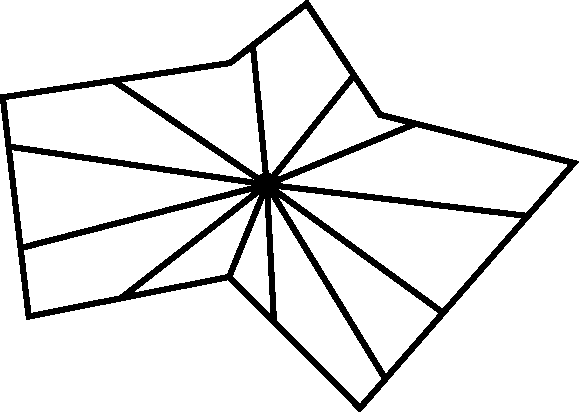
\includegraphics[width=3cm]{3_40}
		\end{wrapfigure}
		
		Ist $ U \subset \R^n $ sternförmig (d.h. $\existss p_0 \in U$, sodass alle geraden Verbindungsstrecken von $p_0$ zu beliebigen Punkten $p$ ganz in $U$ enthalten sind), dann ist jede geschlossene Form auf $U$ exakt.
	\end{minipage}
\end{thm}

\begin{exmp*}
	Die geschlossene, auf $\R^2 \setminus \{0\}$ nicht exakte Form $ \alpha = \frac{1}{x^2+y^2}(ydx-xdy) $ ist auf $ \{(x,y) \in \R^2 \mid x > 0\} $ exakt ($ f = \tan^{-1} \frac{y}{x} $)
\end{exmp*}

\begin{cor}
	Ist $ \omega \in \Omega^1(M)$ geschlossen, so besitzt jeder Punkte $ p \in M $ eine Umgebung, auf der $\omega$ exakt ist.
\end{cor}